%======================================================================
\subsection{Unstable manifolds and shadowing}

% ----------------------------------------------------------------------
\begin{frame}
  \frametitle{\On{2} symmetry reduction}
  \putsymf

  \begin{center}
    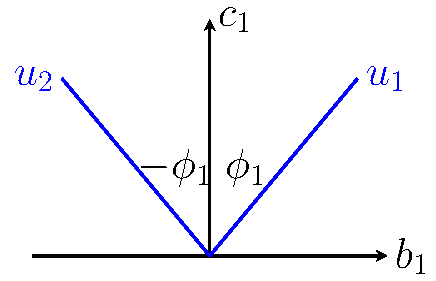
\includegraphics[width=0.4\textwidth]{sliceAngle}
  \end{center}

  \htb{Fundamental domain} in the slice:
  \begin{equation}
    \label{eq:fundDomain}
    \hat{b}_2 > 0
    \,.
  \end{equation}
  

\end{frame}

% ----------------------------------------------------------------------
\begin{frame}%[allowframebreaks]
  \frametitle{Unstable manifold of \EQV{2}}
  
  {\centering
    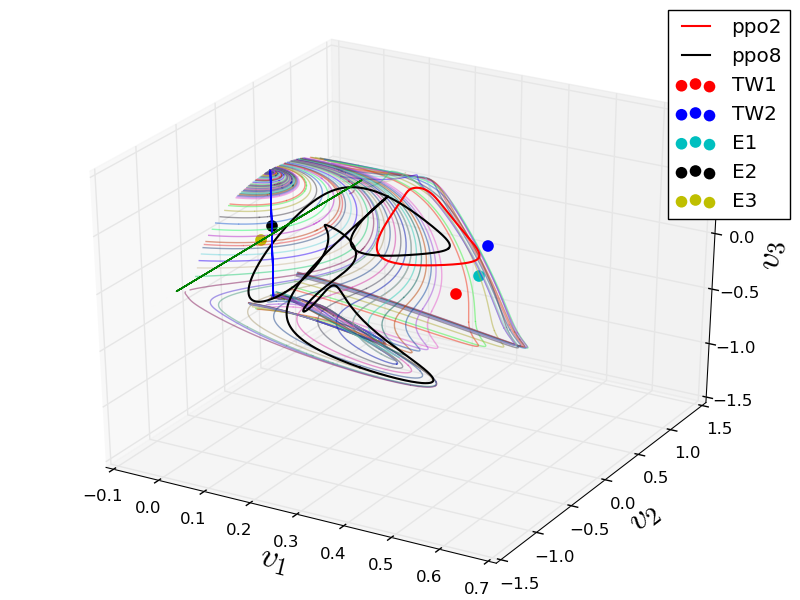
\includegraphics[width=0.7\textwidth]{ppo8}
  \par}
  { \scriptsize 
    The dense set of thin curves is the unstable
    manifold of \EQV{2}.  The blue and green straight lines are the group orbits of
    \EQV{2} and \EQV{3} respectively. 
    \texttt{ppo2} is \PPO{14.33}.
    \texttt{ppo8} is \PPO{41.08}.
    $[v_1, v_2, v_3] = [\hat{c}_1, \hat{c}_3, \hat{c}_2]$. 
  }
  
\end{frame}

% ----------------------------------------------------------------------
% \begin{frame}%[allowframebreaks]
%   \frametitle{Unstable manifold of \EQV{2}}

%   {\centering
%     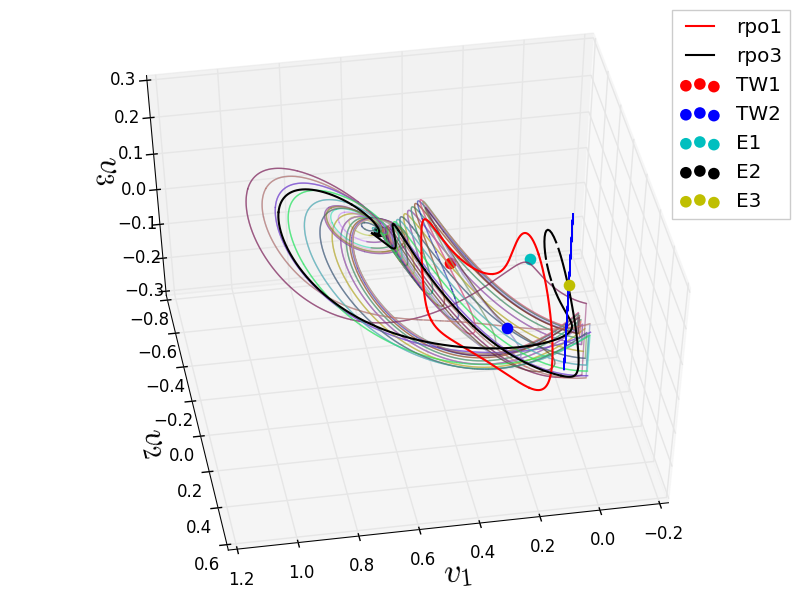
\includegraphics[width=0.7\textwidth]{rpo3}
%     \par}
%   { \scriptsize 
%     The dense set of thin curves is the unstable
%     manifold of \EQV{2}. 
%     The blue and green straight lines are the group orbits of
%     \EQV{2} and \EQV{3} respectively.
%     \texttt{rpo1} is \RPO{16.31}.
%     \texttt{rpo3} is \RPO{33.50}.
%     $[v_1, v_2, v_3] = [\hat{c}_1, \hat{c}_3, \hat{c}_2]$. 
%   }

% \end{frame}

% ----------------------------------------------------------------------
\begin{frame}%[allowframebreaks]
  \frametitle{Shadowing among orbits}
  
  {\centering
    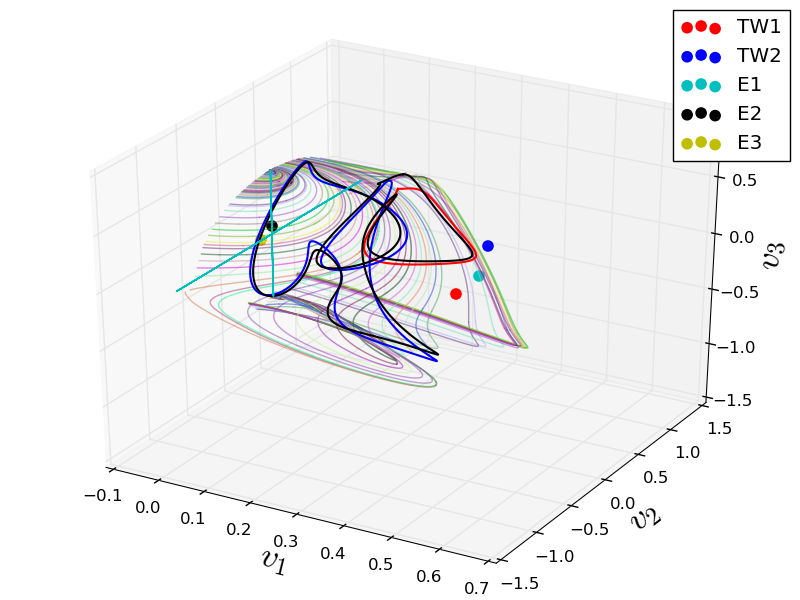
\includegraphics[width=0.75\textwidth]{rpo1rpo5rpo22Im} 
    \par}
  {\scriptsize 
    (red) \RPO{16.31}, (blue) \RPO{35.97}
    and (black) \RPO{57.59}. 
  }

\end{frame}

% ----------------------------------------------------------------------
% \begin{frame}%[allowframebreaks]
%   \frametitle{Shadowing among orbits}

%   {\centering
%     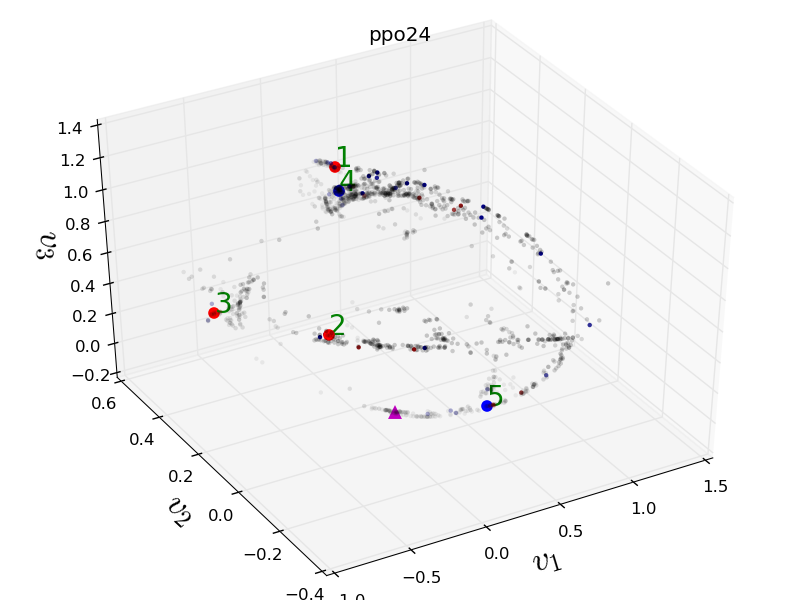
\includegraphics[width=0.75\textwidth]{ppo24}
%     \par}
%   {\scriptsize
%     The red is \texttt{ppo2} (\PPO{14.33}).
%     The black is \texttt{ppo24} (\PPO{57.67}).
%   }
%\end{frame}
